\documentclass[xcolor=dvipsnames]{beamer} 
\usepackage{ulem}
\usepackage{tabularx}
\usepackage{xcolor,colortbl}

\newcommand{\mc}[2]{\multicolumn{#1}{c}{#2}}
\definecolor{Gray}{gray}{0.85}
\definecolor{LightGreen}{rgb}{1,0.88,1}

\newcolumntype{a}{>{\columncolor{Gray}} X }
\newcolumntype{b}{>{\columncolor{white}} X }


% This file is a solution template for:

% - Talk at a conference/colloquium.
% - Talk length is about 20min.
% - Style is ornate.



% Copyright 2004 by Till Tantau <tantau@users.sourceforge.net>.
%
% In principle, this file can be redistributed and/or modified under
% the terms of the GNU Public License, version 2.
%
% However, this file is supposed to be a template to be modified
% for your own needs. For this reason, if you use this file as a
% template and not specifically distribute it as part of a another
% package/program, I grant the extra permission to freely copy and
% modify this file as you see fit and even to delete this copyright
% notice. 


\mode<presentation>
{
  %\usetheme{boxes}
  %\usecolortheme{seagull}
  % or ...

  \setbeamercovered{transparent}
  % or whatever (possibly just delete it)

    \usecolortheme[named=OliveGreen]{structure} 
    \usetheme[height=7mm]{Rochester} 
    \setbeamertemplate{items}[ball] 
    \setbeamertemplate{blocks}[rounded][shadow=true]
}


\usepackage[czech]{babel}
% or whatever

\usepackage[utf8]{inputenc}
% or whatever

\usepackage{hyperref}
%\definecolor{links}{HTML}{2A1B81}
\hypersetup{colorlinks,linkcolor=OliveGreen,urlcolor=OliveGreen}

\usepackage{times}
% \usepackage[T1]{fontenc}
% Or whatever. Note that the encoding and the font should match. If T1
% does not look nice, try deleting the line with the fontenc.



% If you have a file called "university-logo-filename.xxx", where xxx
% is a graphic format that can be processed by latex or pdflatex,
% resp., then you can add a logo as follows:

\pgfdeclareimage[height=1.cm]{conference-logo}{images/IGif2004f.jpg}
\pgfdeclareimage[height=1.cm]{ol-logo}{images/openlayers.png}
\pgfdeclareimage[height=1.cm]{ol3-logo}{images/ol3.png}
\pgfdeclareimage[height=1.cm]{leaflet-logo}{images/leaflet.png}
\logo{\pgfuseimage{conference-logo}}



% Delete this, if you do not want the table of contents to pop up at
% the beginning of each subsection:
%\mode<presentation>
%\AtBeginSection[]
%{
%%\logo{\pgfuseimage{conference-logo}}
%  \begin{frame}<beamer>{TOC}
%    \tableofcontents[currentsection,currentsubsection]
%  \end{frame}
%}


% If you wish to uncover everything in a step-wise fashion, uncomment
% the following command: 

%\beamerdefaultoverlayspecification{<+->}


\title{Občanské sdružení Otevřená GeoInfrastruktura}

\subtitle {}

\author[J. Čepický] % (optional, use only with lots of authors)
{Jáchym~Čepický\inst{1}}
% - Give the names in the same order as the appear in the paper.
% - Use the \inst{?} command only if the authors have different
%   affiliation.

\institute % (optional, but mostly needed)
{
  \inst{1}%
  OSGeo.cz
  \url{http://osgeo.cz}\\
}
  
% - Use the \inst command only if there are several affiliations.
% - Keep it simple, no one is interested in your street address.

\date[GIS Ostrava 2014] % (optional, should be abbreviation of conference name)
{GIS Ostrava 2014}
% - Either use conference name or its abbreviation.
% - Not really informative to the audience, more for people (including
%   yourself) who are reading the slides online



\begin{document}

%\begin{abstract}
%\end{abstract}

\begin{frame}
  \titlepage
\end{frame}

\begin{frame}{TOC}
  \tableofcontents
  % You might wish to add the option [pausesections]
\end{frame}


% Structuring a talk is a difficult task and the following structure
% may not be suitable. Here are some rules that apply for this
% solution: 

% - Exactly two or three sections (other than the summary).
% - At *most* three subsections per section.
% - Talk about 30s to 2min per frame. So there should be between about
%   15 and 30 frames, all told.

% - A conference audience is likely to know very little of what you
%   are going to talk about. So *simplify*!
% - In a 20min talk, getting the main ideas across is hard
%   enough. Leave out details, even if it means being less precise than
%   you think necessary.
% - If you omit details that are vital to the proof/implementation,
%   just say so once. Everybody will be happy with that.

\section{}
\begin{frame}
\begin{itemize}
    \item Občanské sdružení Otevřená GeoInfrastruktura\footnote{Podle
    ,,starého`` občanského zákoníku}
    \item Ustavující členské schůze 15.1.2014
    \item \url{http://osgeo.cz}
\end{itemize}
\end{frame}

\begin{frame}{Stanovy}
\begin{center}
    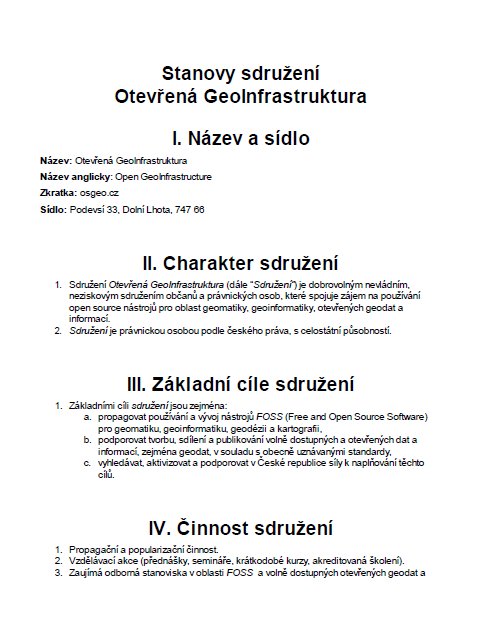
\includegraphics[width=0.5\textwidth]{imgs/stanovyI.png}
    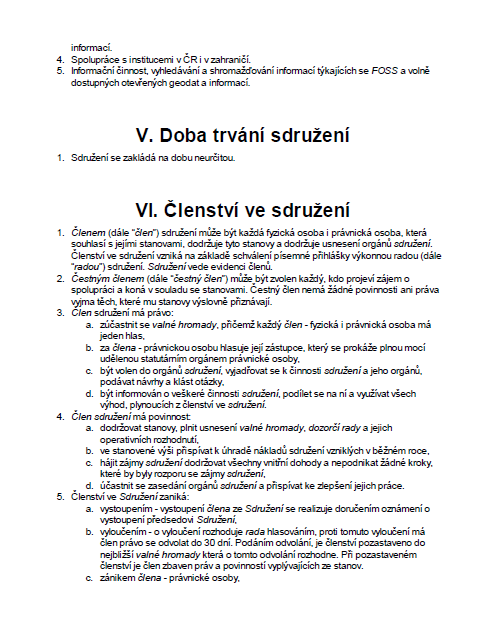
\includegraphics[width=0.5\textwidth]{imgs/stanovyII.png}\\
    \url{http://goo.gl/K85SzB}
\end{center}
\end{frame}

\begin{frame}{Stanovy}
\begin{itemize}[<+->]
    \item Propagovat používání a vývoj nástrojů FOSS (Free and Open Source
    Software) pro geomatiku, geoinformatiku, geodézii a kartografii
    \item \alert{Podporovat tvorbu, sdílení a publikování volně dostupných a
    {\em otevřených} dat a informací, zejména geodat, v souladu s obecně uznávanými
    \emph{standardy}}
    \item Vyhledávat, aktivizovat a podporovat v České republice síly k
    naplňování těchto cílů
\end{itemize}
\end{frame}

\begin{frame}{Otevřená data\footnote{http://opendata.cz/cs/node/29}}
\begin{description}[<+->]
    \item[Technická otevřenost:] zveřejnění dat ve standardním strojově čitelném formátu
    \item[Legislativní otevřenost:] zveřejnění dat pod otevřenou licencí
    \item[Dostupnost a původnost:] jednotlivé datové sady jsou zveřejňovány jako jeden celek a nezměněné (tj. např. ne statistiky ale data, na základě kterých se dají statistiky spočítat)
    \item[Přehlednost:] katalogizace datových sad v katalogu dat pro usnadnění vyhledávání
\end{description}
\end{frame}

\begin{frame}{GeoInfostrategie\footnote{Záměr vypracování Strategie rozvoje
    infrastruktury pro prostorové informace v České republice do roku 2020}: Vize ČR 2020}
 Česká republika je znalostní společností účelně využívající prostorové informace. 
\begin{itemize}
    \item Prostorové informace a související služby jsou využívány ve
        všech oblastech života společnosti a podporují konkurenceschopnost,
        bezpečnost, sociální soudržnost a trvale udržitelný rozvoj.
    \item Veřejný sektor díky dostupnosti prostorových informací a služeb
        efektivně poskytuje moderní a kvalitní veřejné služby. 
\end{itemize}
Nastavení jasných pravidel pro efektivní a koordinovanou tvorbu, správu,
využívání a \emph{otevřené sdílení prostorových informací} ve veřejné správě a jejich
co nejširší \emph{využívání celou společností}.
\end{frame}

\begin{frame}{Více informací}
\begin{itemize}
    \item \url{http://osgeo.cz}
    \item Dnes po ,,Přivítacím nápoji`` neformální setkání
    \item stanovy: \url{http://goo.gl/K85SzB}
\end{itemize}
\end{frame}

%\begin{frame}
%    \begin{center}
%        
\includegraphics[width=\textwidth]{imgs/Borg_aboard_Enterprise_(NX-01).jpg}
%    \end{center}
%\end{frame}

\section*{Conclusion}
\begin{frame}
    jachym.cepicky@gmail.com \\
    http://osgeo.cz
\end{frame}


\end{document}
